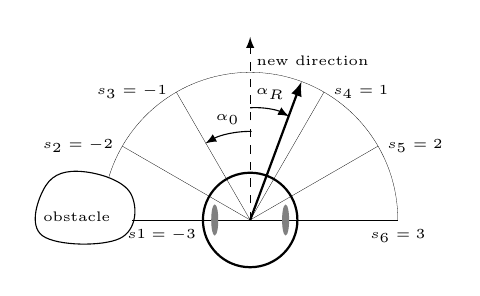
\begin{tikzpicture}[scale=0.75,font=\tiny]

% sensors
\draw [ultra thin, rotate=0](0,0) --  (2.5,0) node[at end, below]{$s_6=3$};
\draw [ultra thin, rotate=30](0,0) --  (2.5,0) node[at end, right]{$s_5=2$};;
\draw [ultra thin, rotate=60](0,0) --  (2.5,0) node[at end, right]{$s_4=1$};;
\draw [ultra thin, rotate=120](0,0) --  (2.5,0) node[at end, left]{$s_3=-1$};;
\draw [ultra thin, rotate=150](0,0) --  (2.5,0) node[at end, left]{$s_2=-2$};;
\draw [ultra thin, rotate=180](0,0) --  (2,0) node[near end, below]{$s1=-3$};;
% direction 
\draw [thick,-latex](0,0) --  (0.8689,2.3417) node[at end, right=4, above=2]{new direction};
% angle
\draw [-latex](0,1.9) arc (93.7723:61.0866:1.2) node[midway,above]{$\alpha_R$};
\draw [-latex](0.0262,1.4998) arc (88.8995:120.3354:1.5) node[midway,above]{$\alpha_0$};

\draw [dashed,-latex](0,0) --  (0,3.1) node[at end, right]{};
% robot
\draw [thick] (0,0) ellipse (0.8 and 0.8);
% wheels
\draw  [fill,gray, rotate around={90:(0.6,0)} ]  (0.6,0) node (v1) {} ellipse (0.25 and 0.05);
\draw  [fill,gray, rotate around={90:(-0.6,0)} ]  (-0.6,0) node (v2) {} ellipse (0.25 and 0.05);
% obstacles
\draw  plot[smooth cycle, tension=.7] coordinates {(-2.0229,0.4472) (-2.8303,0.8188) (-3.4616,0.58) (-3.5145,-0.2685) (-2.2068,-0.3128)} node[below=-8,left]{obstacle};
% \draw  plot[smooth cycle, tension=.7] coordinates {(1.2,0.9) (1.6,0.5) (1.5,-0.2) (2.4,-0.1)  (1.9,1.2)};
%circle
\draw [ultra thin] (2.5,0) arc (0:163:2.5);



\end{tikzpicture}